\documentclass[11pt,a4paper]{article}

\usepackage{amsmath,amssymb}
\usepackage{graphicx}
\usepackage{geometry}
\usepackage{physics}
\usepackage{hyperref}
\usepackage{float}

\usepackage{titling}

\setlength{\droptitle}{-6em}      % moves title up
\posttitle{\par\vspace{-5.5em}}     % space after title

\setlength{\parindent}{0pt}
\setlength{\parskip}{6pt}

\geometry{margin=1in}

\title{\textbf{Analytical Shell Study of an NFW Halo}}
\date{}

\begin{document}

\maketitle

\section{Introduction and motivation}
In collisionless $N$-body simulations of dark matter halos, both inner and outer regions are typically represented using particles; however, the outer halo is generally smoother and less well resolved, which can introduce numerical noise and unnecessary computational expense. To address this, we consider a hybrid model in which the inner halo ($r < r_{\mathrm{cut}}$) is evolved using particles, while the outer halo ($r > r_{\mathrm{cut}}$) is replaced by an analytic gravitational potential. The purpose of this document is to quantify the influence of the outer halo on the inner region and assess whether this simplified treatment can accurately reproduce its gravitational effects.

\section{NFW halo model}

We assume a spherically symmetric Navarro--Frenk--White (NFW) profile:

\begin{equation}
\rho(r) = \frac{\rho_s}{(r/r_s)(1 + r/r_s)^2},
\end{equation}

where $\rho_s$ is the characteristic density and $r_s$ is the scale radius.

The enclosed mass is:

\begin{equation}
M(<r) = 4\pi \rho_s r_s^3 \left[ \ln(1+x) - \frac{x}{1+x} \right], \quad x = \frac{r}{r_s}.
\end{equation}

The halo is truncated at $r_{\mathrm{vir}}$.

The halo is divided into logarithmically spaced spherical shells:

\begin{equation}
r_i \in [r_{\mathrm{min}}, r_{\mathrm{vir}}].
\end{equation}

Each shell is treated independently to evaluate its contribution to mass, potential, and force.

\section{Gravitational potential and force}
The gravitational potential is:

\begin{equation}
\Phi(r) = -\frac{G M(<r)}{r}
- 4\pi G \rho_s r_s^2 \left[ \frac{1}{1 + r/r_s} - \frac{1}{1 + c} \right],
\end{equation}

where $c = r_{\mathrm{vir}} / r_s$.

Unlike the force, the potential depends on all mass, including material at larger radii.

The radial acceleration is:

\begin{equation}
a(r) = \frac{G M(<r)}{r^2}.
\end{equation}

By the shell theorem, only mass inside $r$ contributes to the force.

\section{Key definitions}

The halo is divided into spherical shells with inner and outer radii $r_i$ and $r_{i+1}$. The \emph{enclosed mass}, $M(<r)$, is the total mass contained within radius $r$. For the NFW model it follows the standard analytic form, and it is the quantity used to compute the radial force under spherical symmetry. The \emph{shell mass} is the mass contained between two adjacent shell boundaries, and the \emph{shell mass fraction} is the mass in a given shell divided by the total halo mass. These quantities are used to show how the mass budget is distributed across radius.

The \emph{probe radius}, $r_{\mathrm{probe}}$, is the radius at which the gravitational quantities are evaluated. In the plots, it marks the location where we ask how much of the potential or force is contributed by different parts of the halo. The \emph{cutoff radius}, $r_{\mathrm{cut}}$, defines the boundary of the hybrid model: particles are retained for $r < r_{\mathrm{cut}}$, while the region $r > r_{\mathrm{cut}}$ is represented by an analytic truncated NFW potential.

To quantify the influence of the outer halo, we define the \emph{outer-potential fraction} as
\begin{equation}
f_{\mathrm{outer}}(r_{\mathrm{probe}}, r_{\mathrm{cut}}) =
\frac{\left|\Phi_{>r_{\mathrm{cut}}}(r_{\mathrm{probe}})\right|}
{\left|\Phi(r_{\mathrm{probe}})\right|},
\end{equation}
where $\Phi_{>r_{\mathrm{cut}}}(r_{\mathrm{probe}})$ is the contribution to the potential at $r_{\mathrm{probe}}$ from material outside the cutoff radius, and $\Phi(r_{\mathrm{probe}})$ is the total potential at that radius. This quantity measures how strongly the outer halo contributes to the local potential.

The \emph{cumulative outer fraction beyond $r_{\mathrm{cut}}$} is the integrated version of this idea: it gives the fraction of the total potential depth, or of the summed shell contribution, that arises from all shells exterior to a chosen cutoff radius. This is useful for identifying the radius beyond which the outer halo becomes only a small correction. Finally, the \emph{force contribution} at a probe radius measures the radial acceleration generated by the mass distribution. In a spherically symmetric halo, only mass enclosed within $r_{\mathrm{probe}}$ contributes to the force, whereas material at larger radii contributes to the potential but not to the local acceleration.

\section{Interpretation of the results}

\subsection{Enclosed mass and shell mass fraction}
The enclosed-mass plot shows the expected monotonic NFW growth with radius, while the shell-mass fraction increases toward larger radii. This means that the outer halo contains a substantial part of the total mass budget. The result is qualitatively consistent with the idea that replacing the outer region by a smooth analytic potential can capture an important part of the halo structure without retaining every outer particle.

\begin{figure}[H]
    \centering
    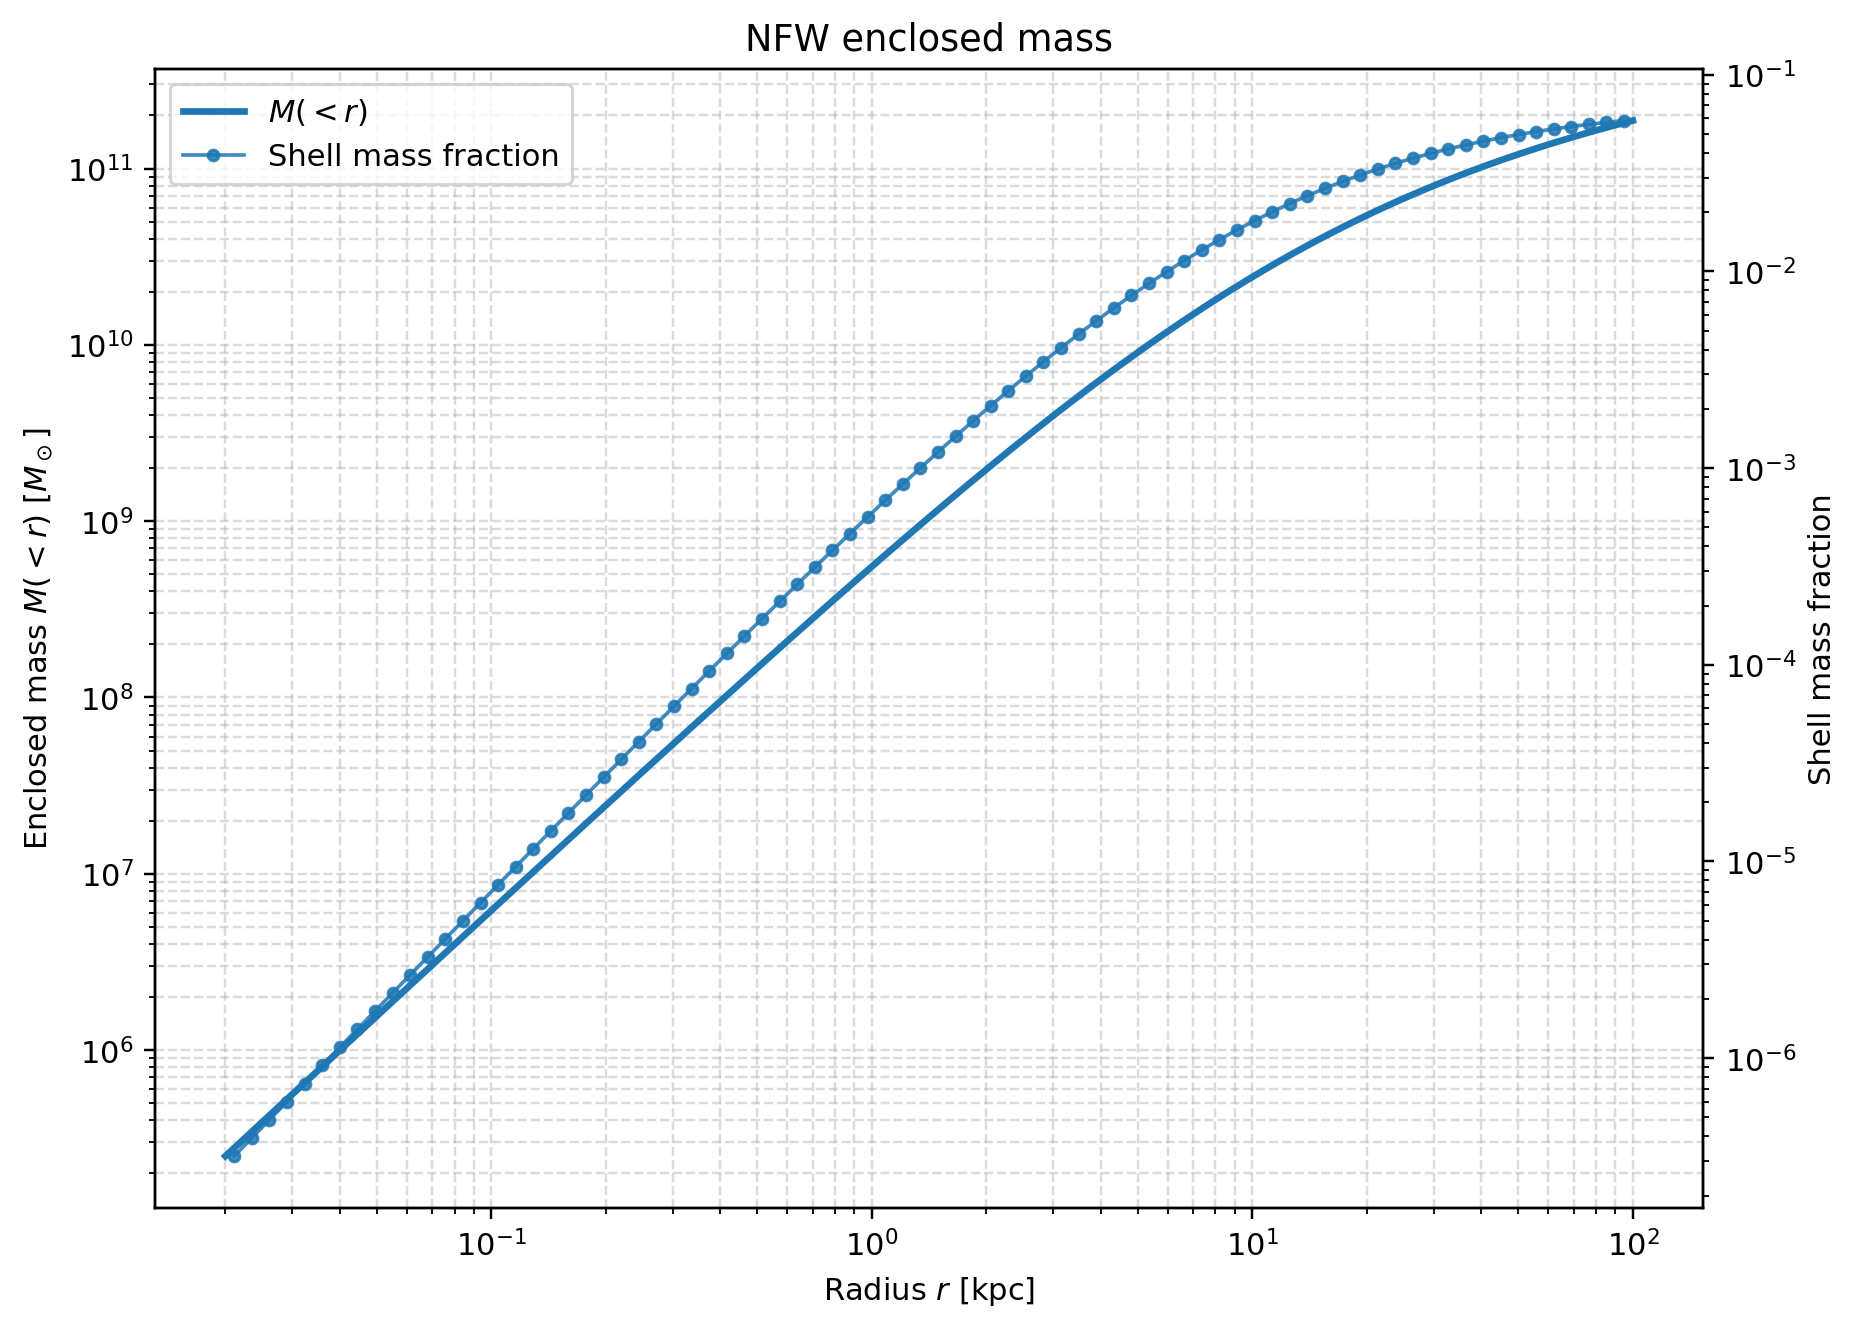
\includegraphics[width=0.7\textwidth]{01_mass_profile_and_shell_fraction.png}
\end{figure}

\subsection{Central potential contribution}
The central-potential plot shows that shells at radii well outside the centre still make a sizeable contribution to the potential depth at $r = 0$. This is exactly what is expected for a spherical halo: outer matter does not change the force at the centre, but it does deepen the potential well and therefore changes the escape-speed scale. The result supports the statement that the inner halo is influenced by the outer halo through the potential background.

\begin{figure}[H]
    \centering
    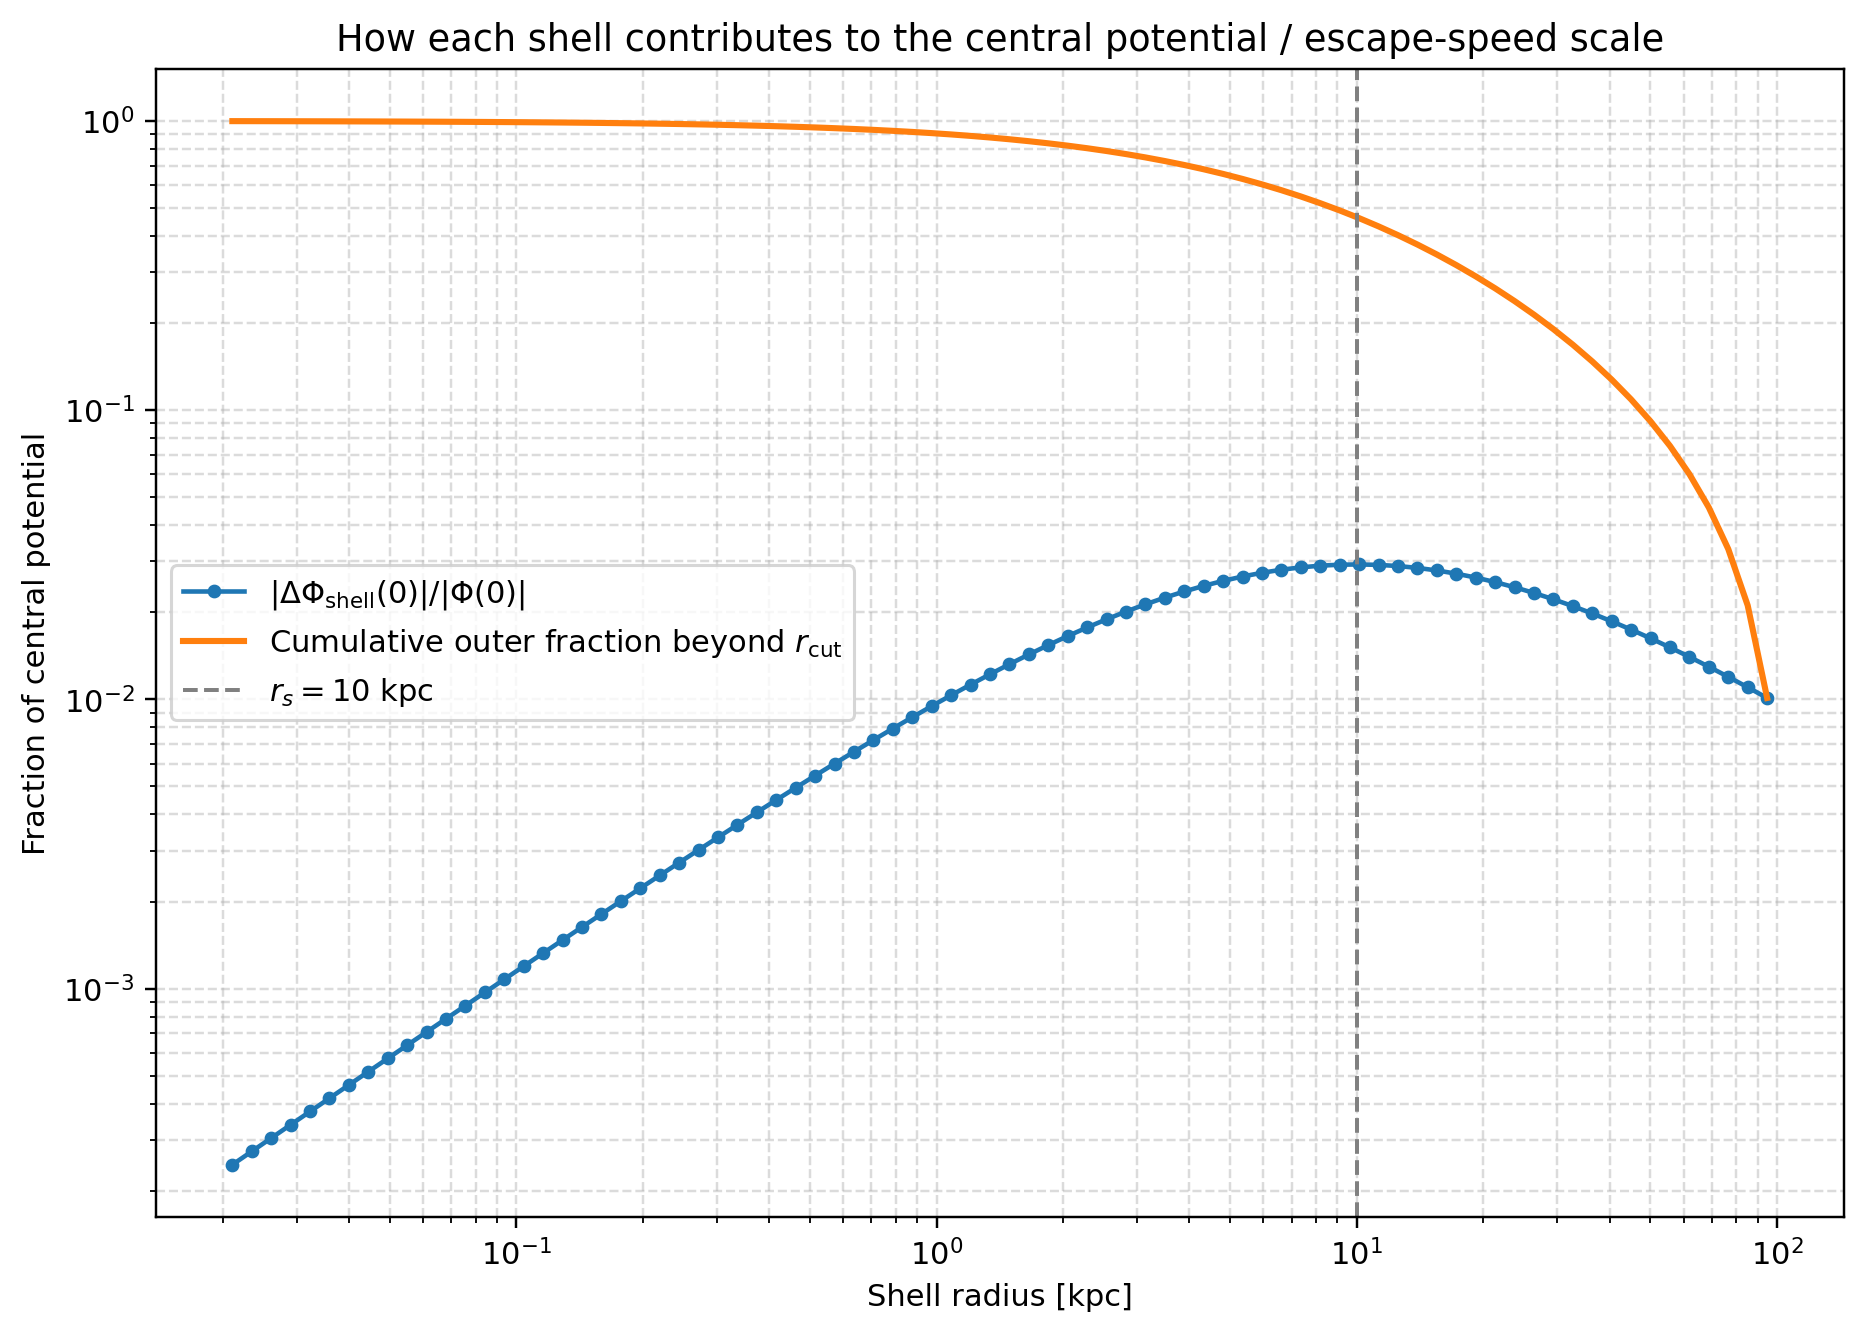
\includegraphics[width=0.7\textwidth]{02_central_potential_shell_contribution.png}
\end{figure}

\subsection{Outer-potential fraction as a function of cutoff radius}
The cutoff-radius plot shows that the fraction of the potential coming from material outside $r_{\mathrm{cut}}$ decreases as the cutoff is moved outward. This is the key diagnostic for selecting a truncation radius. If the outer-potential fraction remains large for the inner radii of interest, then the outer halo cannot be ignored or replaced by a crude boundary. Instead, it should be represented by a smooth analytic component.

\begin{figure}[H]
    \centering
    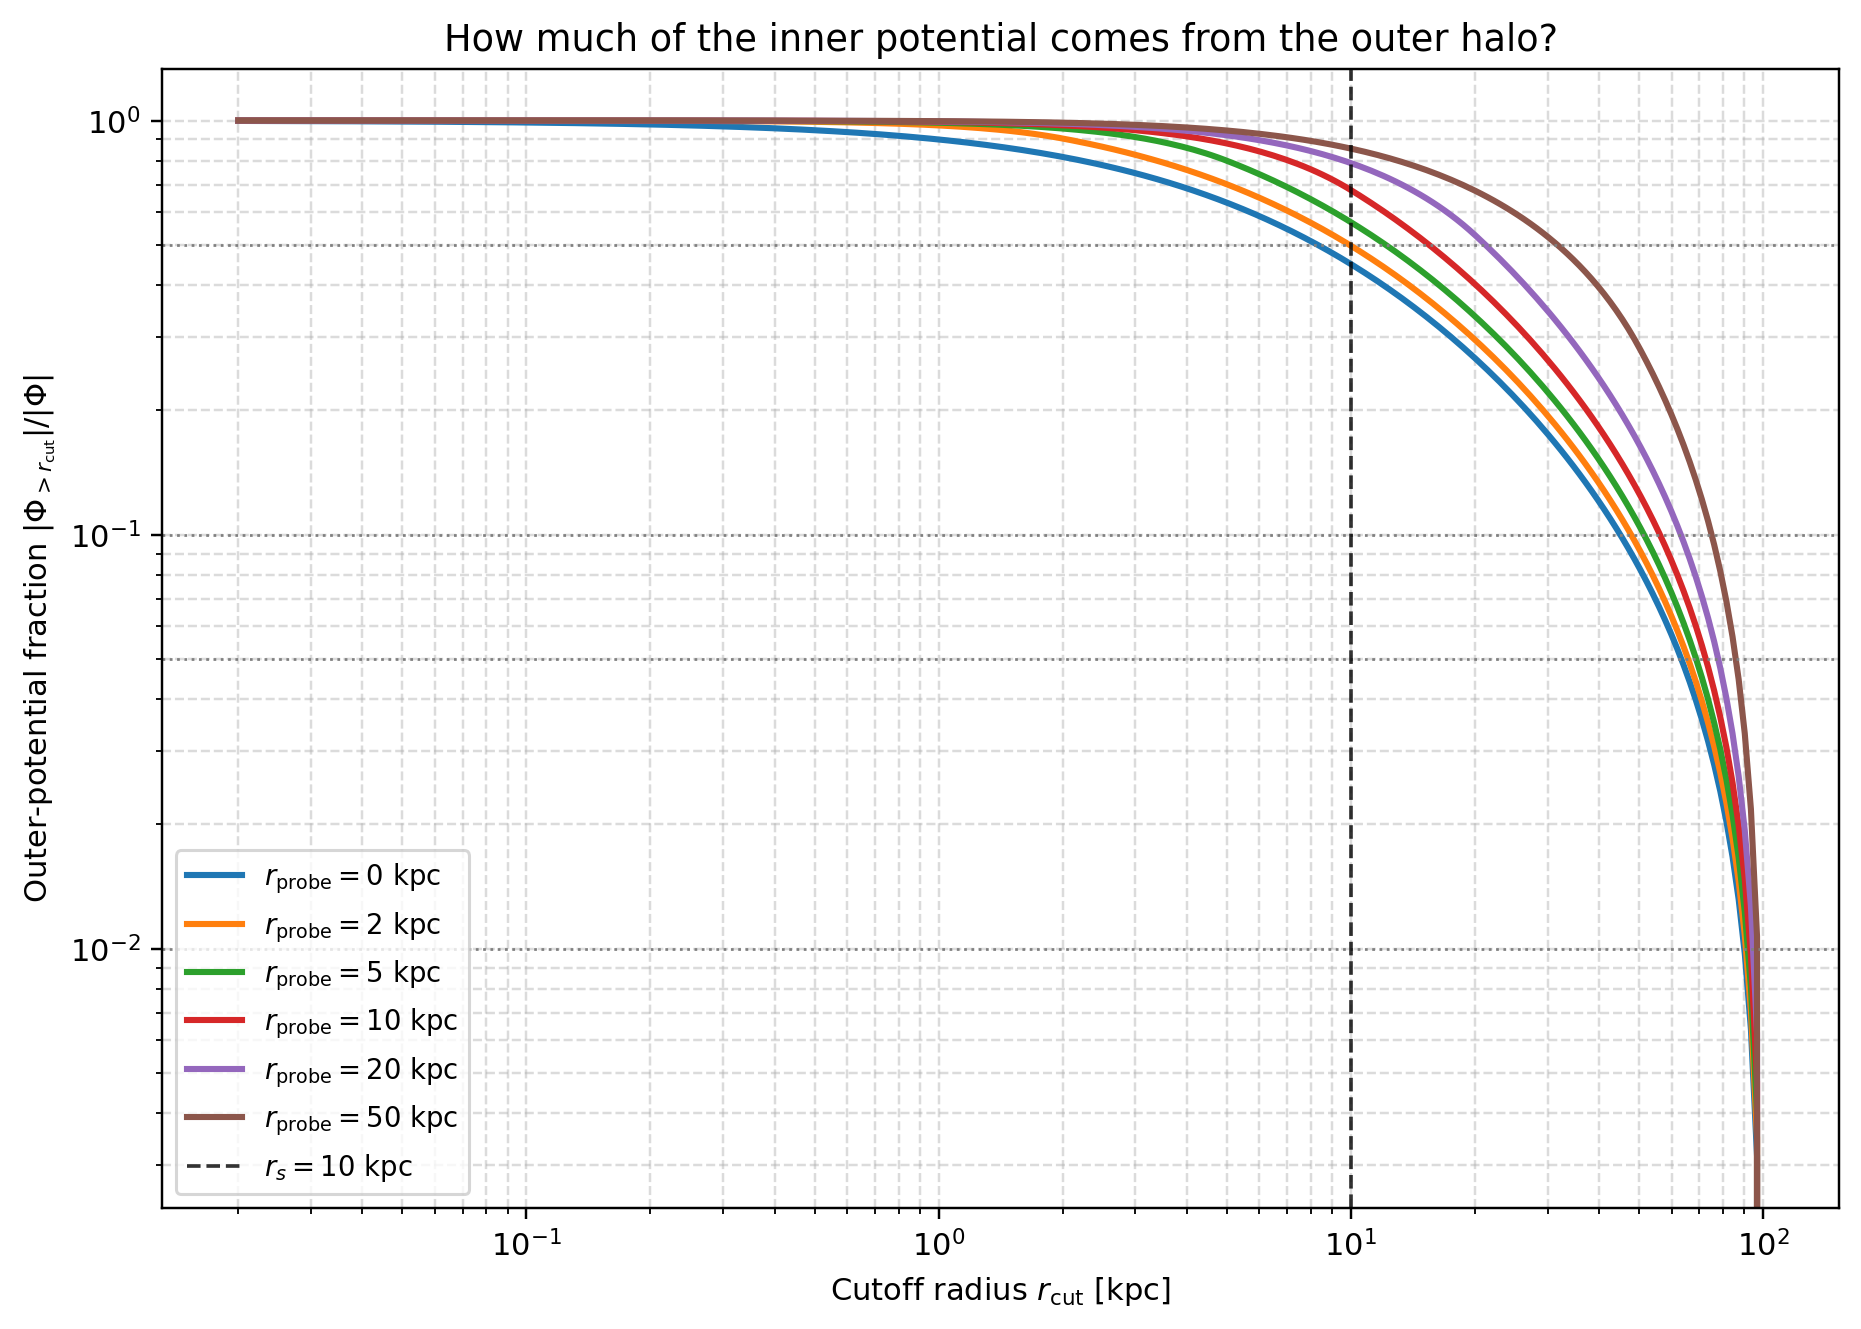
\includegraphics[width=0.7\textwidth]{03_outer_fraction_vs_cutoff.png}
\end{figure}

\subsection{Outer-fraction map}

The 2D map of the outer-potential fraction provides a compact summary of the same physical effect. It shows that for small values of $r_{\mathrm{cut}}$, the outer halo contributes significantly to the potential across a wide range of probe radii. This contribution becomes negligible only when the cutoff radius approaches the outer extent of the halo.

This visualization is particularly useful for selecting a practical value of $r_{\mathrm{cut}}$ that ensures the outer halo contribution is sufficiently small within the region of interest.

\begin{figure}[H]
    \centering
        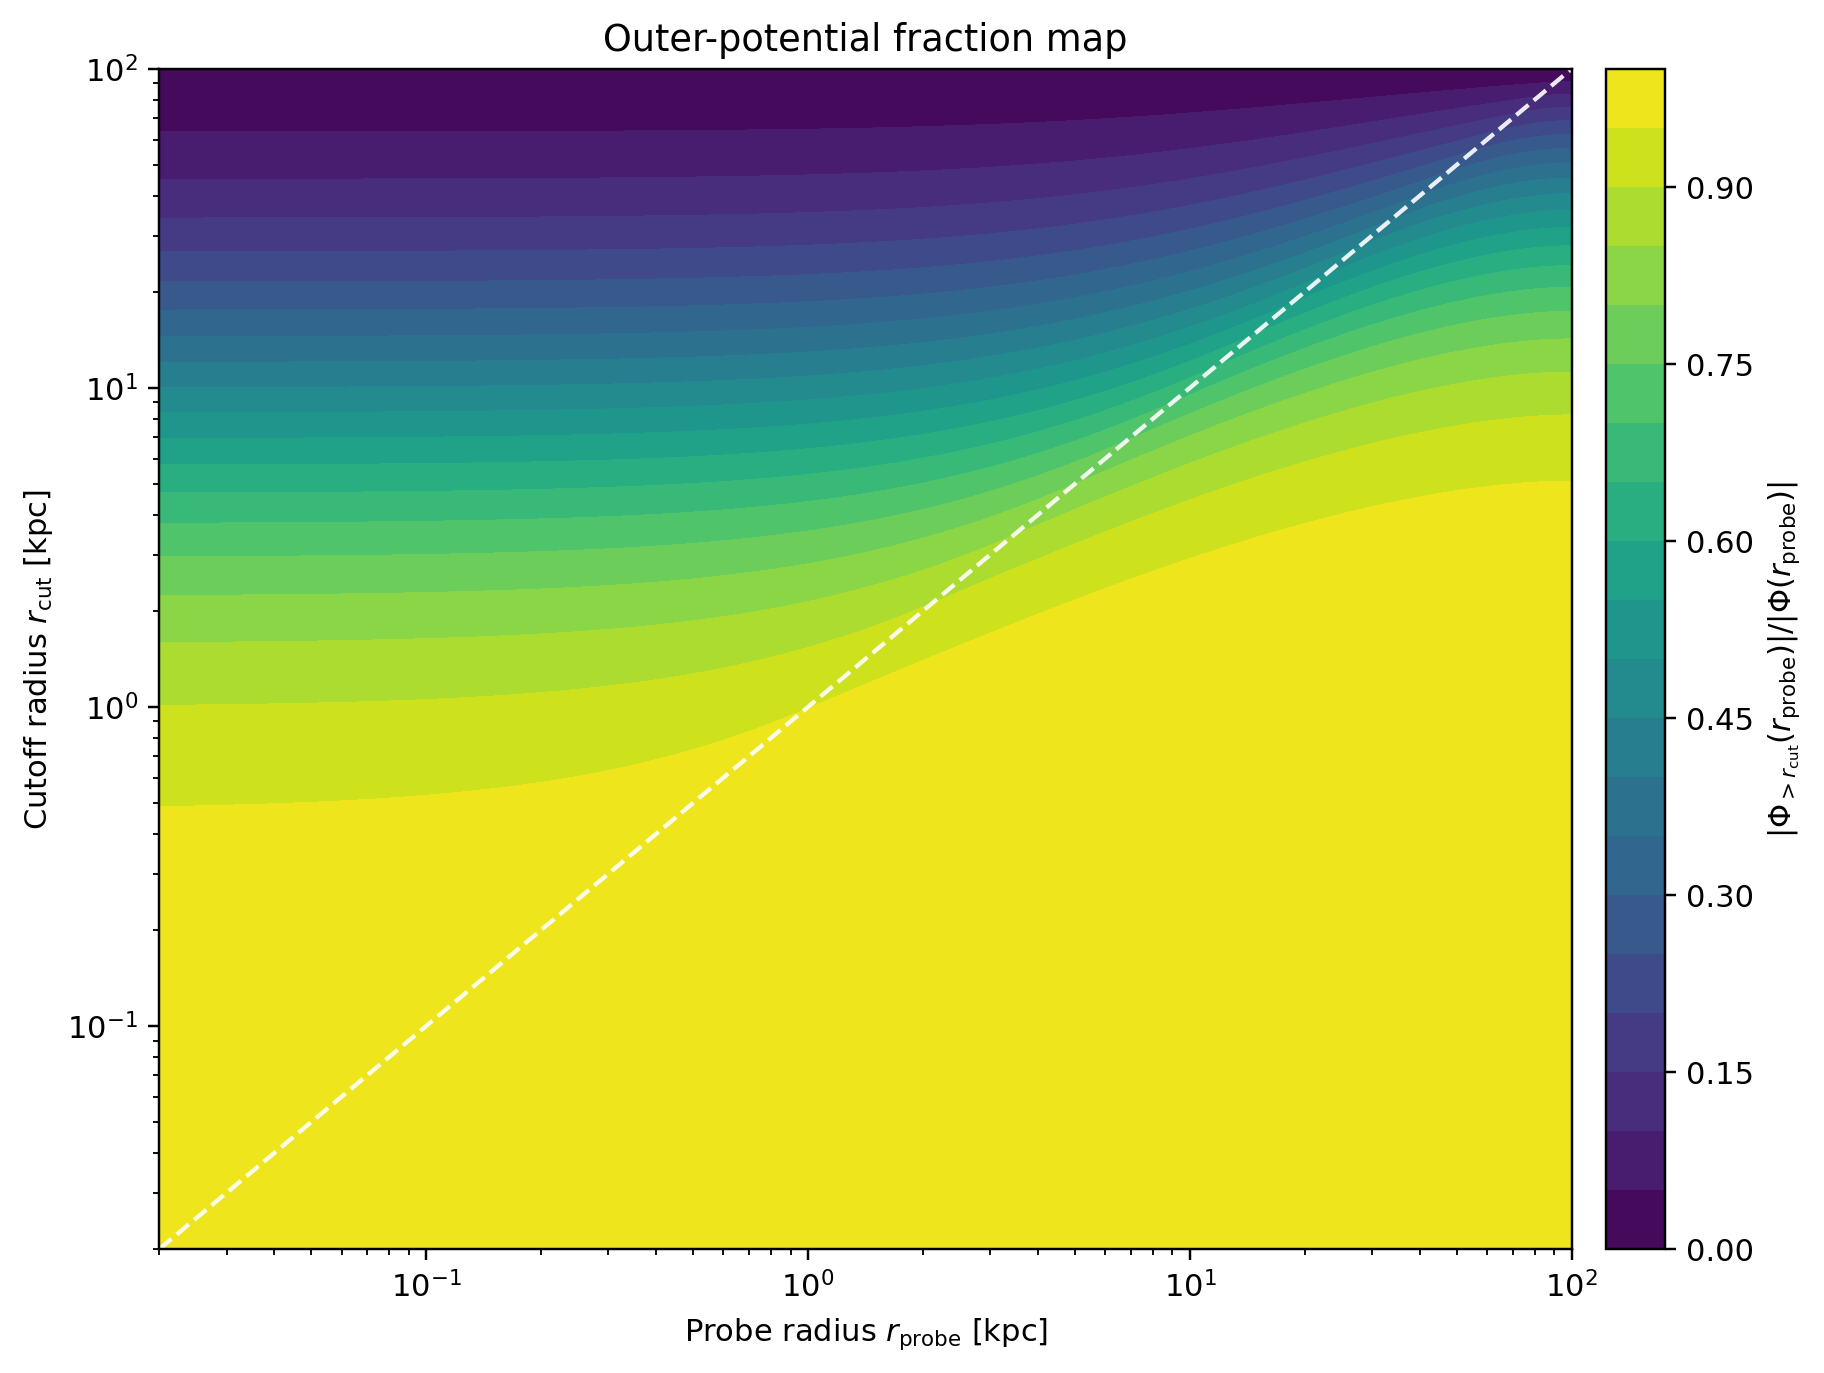
\includegraphics[width=0.7\textwidth]{04_outer_fraction_map.png}
\end{figure}



\end{document}